\chapter{Results}
    \label{cha:results}
    %
    \section{Non-cooperative enzymes do not entail bistable systems}
        \label{sec:ResNon-cooperative}
        %
        In this section, we consider a system without cooperative enzymes. Thus, all the enzymes in the system read nucleosomes with a distance of 1 from the nucleosome that is written on. It is important to point out, that the nucleosome which is modified is included in the context as well.
        %

        %
        Thanks to Mayer's pionous work \cite{mayer2020langevin}, there were already some presumptions available that allowed to start from an educated guess. As pointed out before, bistability can not be achieved in such a system.\\
        %
        \begin{figure}[!htbp]
            \centering
            \includerunplot{Results/3.1_noncoopNotBistable/longRun_nonCyclic_highDiss_2_runHistoryPlot.pdf}
            \caption{Absolute number of nucleosome states (active in green, silent in red) during the course of one long simulation (about 3.9 million reaction steps). The enzyme rule set contains linear extenders, linear removers, random adders and random removers. The rule set does not contain cooperative enzymes. {\color{red} (Rates and additional runs can be found in Appendix?)\color{black}}}
            \label{img:nonCoopSim}
        \end{figure}
        %
        % TODO: Do calculations completely without linear extenders as well as with extremely strong linear extenders
        %
        Looking at fig. \ref{img:nonCoopSim}, the nucleosome string states achieved during the simulation indeed disclose a monostable system. Accordingly, the histogram which counts the occurrence of active and silent nucleosomes respectively within the string  shows a unimodal distribution throughout the simulation.
        %
        Fig. \ref{img:nonCoopSim} exemplarily shows that the total number of active and silent states ambulate around one same value. Although susceptible to some variance, this value can, throughout all simulations that were done, be approximated to 30, which is half of the totality of nucleosomes in the system. % TODO put more of these simulations into appendix?
        %

        %
        On a sidenote, it should be mentioned that, in order to guarantee reproducibility and truthfulness of the statements derived from the plots, it was always made sure, that the state distribution indicated by the histograms in the plots were as close to each other as possible. However, in some cases, this goal could not be achieved, as can be seen here. The impact of this issue will be evaluated in section \ref{cha:discussion}.\\
        %

        %
        \begin{figure}[htpb!]
            \centering
            \includeheatmap{Results/3.1_noncoopNotBistable/shortRun_nonCyclic_highDiss_bindingNumbers_5runs_numberAnnot.pdf}
            \vspace{.3cm}
            \begin{center}
                \begin{tabular}{l l}
                    \hline
                    \textbf{\#} & \textbf{enzyme type} \\
                    \hline
                    $[\ 0]$: & linear adder ac to right \\
                    $[\ 1]$: & linear adder ac to left \\
                    $[\ 2]$: & linear adder me to right \\
                    $[\ 3]$: & linear adder me to left \\
                    $[\ 4]$: & linear remover ac to right \\
                    $[\ 5]$: & linear remover ac to left \\
                    $[\ 6]$: & linear remover me to right \\
                    $[\ 7]$: & linear remover me to left \\
                    $[\ 8]$: & random adder ac \\
                    $[\ 9]$: & random adder me \\
                    $[10]$: & random remover me \\
                    $[11]$: & random remover ac \\
                    \hline
                \end{tabular}
            \end{center}
            \caption{Heatmap depicting the absolute numbers of enzyme associations per enzyme and per nucleosome on the nucleosome string. The numbers were summed up over 5 simulations, where each run was simulated over 750,000 time steps on average.}
            \label{img:nonCoopAssocHeatmap}
        \end{figure}
        %

        %
        As can be seen in fig. \ref{img:nonCoopAssocHeatmap}, every enzyme type shows somewhat, in some cases tremendously, different degrees of activity. Also, the distribution of the association events for one enzyme is not uniform. It can clearly be seen that for the linear extenders, the linear removers and the random adders, the enzymatic activity is lower on the string borders. Given that the linear extenders and removers merely have a context reach of 1 (next-neighbour reach) and random adders do not have any reach at all, the lower border activity is an interesting property of the overall system. The fact that the very first nucleosome on the string does not bind any enzymes that have a reading context to the left (with convention of reading from nucleosome 1 on the left to nucleosome 60 on the right) naturally was to be expected. This phenomenon is also observable on the last nucleosome with enzymes which have a reading context to the right.
        %

        %
        \begin{itemize}
            {
                \color{red}
                \item print (not plot) the total step number and indicate it in the caption
                \item include more graphs into appendix
            }
        \end{itemize}
        %
    %
    %
    \newpage
    \section{Bistability on a non-cyclic nucleosome string}
        \label{sec:ResNonCyc}
        %
        \subsection{Impact of cooperative enzymes}
            %
            Contrarily to section \ref{sec:ResNon-cooperative}, the simulations described in this section had cooperative adders and removers present in their enzyme sets which, in theory, enables the system to show bistability.
            %

            %
            \begin{figure}[htpb!]
                \centering
                \includerunplot{Results/3.2_nonCyclString/shortRun_nonCyclic_highDiss_wCoopRem_3_runHistoryPlot.pdf}
                \caption{}
                \label{img:nonCyclBistability_runPlot}
            \end{figure}
            %
            \begin{figure}[htpb!]
                \includeheatmap{Results/3.2_nonCyclString/shortRun_nonCyclic_highDiss_wCoopRem_3_bindingNumbers_numberAnnot.pdf}
                    \vspace{.3cm}
                    \begin{center}
                    \small
                    \begin{minipage}{.49\textwidth}
                        \begin{tabular}{l l}
                            \hline
                            \textbf{\#} & \textbf{enzyme type} \\
                            \hline
                            $[\ 0]$: & coop. adder ac space=0 \\
                            $[\ 1]$: & coop. adder ac space=1 \\
                            $[\ 2]$: & coop. adder ac space=2 \\
                            $[\ 3]$: & coop. adder ac space=3 \\
                            $[\ 4]$: & coop. adder ac space=4 \\
                            $[\ 5]$: & coop. adder ac space=5 \\
                            $[\ 6]$: & coop. adder ac space=6 \\\hline
                            $[\ 7]$: & coop. adder me space=0 \\
                            $[\ 8]$: & coop. adder me space=1 \\
                            $[\ 9]$: & coop. adder me space=2 \\
                            $[10]$: & coop. adder me space=3 \\
                            $[11]$: & coop. adder me space=4 \\
                            $[12]$: & coop. adder me space=5 \\
                            $[13]$: & coop. adder me space=6 \\\hline
                            $[14]$: & coop. remover ac space=0 \\
                            $[15]$: & coop. remover ac space=1 \\
                        \end{tabular}
                    \end{minipage}
                    \hfill
                    \begin{minipage}{.49\textwidth}
                        \begin{tabular}{l l}
                            $[16]$: & coop. remover ac space=2 \\
                            $[17]$: & coop. remover ac space=3 \\
                            $[18]$: & coop. remover ac space=4 \\
                            $[19]$: & coop. remover ac space=5 \\
                            $[20]$: & coop. remover ac space=6 \\\hline
                            $[21]$: & coop. remover me space=0 \\
                            $[22]$: & coop. remover me space=1 \\
                            $[23]$: & coop. remover me space=2 \\
                            $[24]$: & coop. remover me space=3 \\
                            $[25]$: & coop. remover me space=4 \\
                            $[26]$: & coop. remover me space=5 \\
                            $[27]$: & coop. remover me space=6 \\\hline
                            $[28]$: & random adder ac \\
                            $[29]$: & random adder me \\
                            $[30]$: & random remover me \\
                            $[31]$: & random remover ac \\
                            \hline \hline
                        \end{tabular}
                    \end{minipage}
                \end{center}

                % \end{center}
                \caption{Heatmap depicting the absolute numbers of enzyme associations per enzyme and per nucleosome on the nucleosome string. The numbers originate from the simulation plotted in fig. \ref{img:nonCyclBistability_runPlot}.}
                \label{img:nonCyclBistability_bindingNumbers}
            \end{figure}
            %
            %
            \begin{figure}[htpb!]
                \centering
                \includeheatmap{Results/3.2_nonCyclString/shortRun_nonCyclic_highDiss_wCoopRem_3_bindingTimeDuration_numberAnnot.pdf}
                \vspace{.3cm}
                \begin{center}
                \small
                \begin{minipage}{.45\textwidth}
                    \begin{tabular}{l l}
                        \hline
                        \textbf{\#} & \textbf{enzyme type} \\
                        \hline
                        $[\ 0]$: & coop. adder ac space=0 \\
                        $[\ 1]$: & coop. adder ac space=1 \\
                        $[\ 2]$: & coop. adder ac space=2 \\
                        $[\ 3]$: & coop. adder ac space=3 \\
                        $[\ 4]$: & coop. adder ac space=4 \\
                        $[\ 5]$: & coop. adder ac space=5 \\
                        $[\ 6]$: & coop. adder ac space=6 \\\hline
                        $[\ 7]$: & coop. adder me space=0 \\
                        $[\ 8]$: & coop. adder me space=1 \\
                        $[\ 9]$: & coop. adder me space=2 \\
                        $[10]$: & coop. adder me space=3 \\
                        $[11]$: & coop. adder me space=4 \\
                        $[12]$: & coop. adder me space=5 \\
                        $[13]$: & coop. adder me space=6 \\\hline
                        $[14]$: & coop. remover ac space=0 \\
                        $[15]$: & coop. remover ac space=1 \\
                    \end{tabular}
                \end{minipage}
                \hfill
                \begin{minipage}{.45\textwidth}
                    \begin{tabular}{l l}
                        $[16]$: & coop. remover ac space=2 \\
                        $[17]$: & coop. remover ac space=3 \\
                        $[18]$: & coop. remover ac space=4 \\
                        $[19]$: & coop. remover ac space=5 \\
                        $[20]$: & coop. remover ac space=6 \\\hline
                        $[21]$: & coop. remover me space=0 \\
                        $[22]$: & coop. remover me space=1 \\
                        $[23]$: & coop. remover me space=2 \\
                        $[24]$: & coop. remover me space=3 \\
                        $[25]$: & coop. remover me space=4 \\
                        $[26]$: & coop. remover me space=5 \\
                        $[27]$: & coop. remover me space=6 \\\hline
                        $[28]$: & random adder ac \\
                        $[29]$: & random adder me \\
                        $[30]$: & random remover me \\
                        $[31]$: & random remover ac \\
                        \hline \hline
                    \end{tabular}
                \end{minipage}
            \end{center}
                \caption{Heatmap depicting the average enzyme binding duration per enzyme and per nucleosome on the nucleosome string. The duration is defined as the number of time steps the enzyme has bound to one and the same nucleosome without dissociation event taking place in between. The numbers originate from the simulation plotted in fig. \ref{img:nonCyclBistability_runPlot}.}
                \label{img:nonCyclBistability_bindingTimeDuration}
            \end{figure}
            %

            %
            Figs. \ref{img:nonCyclBistability_runPlot}, \ref{img:nonCyclBistability_bindingNumbers} and \ref{img:nonCyclBistability_bindingTimeDuration} are derived from a model containing the two cooperative enzyme types.
            %

            %
            One can easily see in fig. \ref{img:nonCyclBistability_runPlot} that the newly added enzymes seem to stabilize the predominant state (here the silencing one). It was found in additional simulation runs (see appendix \ref{app:additionalRuns}) that the active state could just as easily turn out as the predominant state for the entire run. This fact seems rather logical as the starting state is a completely unmodified string and the enzyme set that is used is purely symmetrical, which means that it does not lean towards any of the two states. The fact that the system can either stably find itself in a completely active as well as a completely silent state shows that bistability has been achieved with this enzyme set.\\
            %

            %
            Figs. \ref{img:nonCyclBistability_bindingNumbers} and \ref{img:nonCyclBistability_bindingTimeDuration} provide more insights into the underlying mechanisms of the system. They are using the same data as fig. \ref{img:nonCyclBistability_runPlot} does. As for the notion of 'space' indicated for each cooperative enzyme, please refer to section \ref{subsubsec:coopEnzymes}. A few seemingly surprising factors are to be addressed here.
            %

            %
            Every single enzyme type shows a trapeze-like shape originating from a decreasing writeable area on the string with increasing context reach. This observation is tied to the inability of the enzymes to look beyond the string borders. As the context size increases, the enzyme is more and more unable to write onto a nucleosome  increasingly further away from the border. This is an unwanted effect, as it does not reflect any behaviour that could be found in nature.
            %

            %
            Fig. \ref{img:nonCyclBistability_bindingTimeDuration} reveals that there is a big discrepancy between the binding time of some enzymes compared to others. As the dissociation rates of the enzymes are very high and, importantly, totally equal for every enzyme, darker spots must mean, that no enzyme has been active on that specific nucleosome at all. For instance, the cooperative acetylation adders only seem to have been active on some nucleosomes close to both borders. Referring to fig. \ref{img:nonCyclBistability_runPlot}, it does not seem surprising that the cooperative acetylation adders and the cooperative methylation removers show relatively low activity as the methylation mark was predominant throughout the entirety of the simulation, because the mentioned adders and removers are most active the more acetylation marks are already on the string. The interesting activity pattern of those two enzyme types suggests that the acetylation subpopulations that can be seen in fig. \ref{img:nonCyclBistability_runPlot} must have been prevalent at the borders of the string almost exclusively. This is supported by the fact that the random methylation remover shows reduced activity at the borders. It is clear to see that the absolute number of associations of the random methylation remover is quite constant on the most of the nucleosomes. Paired with its context only consisting of the nucleosome it is writing on and the fact that there are no associations without adding the mark to the bound nucleosome, the association number of the random enzyme removers can be taken as a locator of the marks they are removing with quite acceptable efficiency.
            %

            %

            %
        %
        %
        \subsection{Bistable switching}
            %
            Considering the biological implications of the system, it would be much more useful if the system could effectively switch from one state to another within the course of a simulation, i.e. without changing the enzyme types involved or their rates and without resetting the nucleosome string to a completely unmodified string.
            %

            %
            This phenomenon, from here on called bistable switching, could not be observed with the
            %

            %
            % With cooperative removers, no bistable switching can be observed: Figs. \ref{img:nonCyclBistability_runPlot}, \ref{img:nonCyclBistability_bindingNumbers} and \ref{img:nonCyclBistability_bindingTimeDuration}.
            %

            %
            % Without the cooperative removers, frequent bistable switchings are observed with quite a bit of noise, meaning high variance around the bells in the histograms: figs. \ref{img:nonCyclBistability_runPlot2} and \ref{img:nonCyclBistability_runPlot3}
            %
            \begin{figure}[htpb!]
                \centering
                \includerunplot{Results/3.2_nonCyclString/longRun_nonCyclic_highDiss_noCoopRem_1_runHistoryPlot.pdf}
                \caption{}
                \label{img:nonCyclBistability_runPlot2}
            \end{figure}
            %
            \begin{figure}[htpb!]
                \centering
                \includerunplot{Results/3.2_nonCyclString/longRun_nonCyclic_highDiss_noCoopRem_4_runHistoryPlot.pdf}
                \caption{}
                \label{img:nonCyclBistability_runPlot3}
            \end{figure}
            %
            \begin{itemize}
                {
                    \color{red}
                    \item Describe difference between with coop removers and without
                    % \item Describe the heatmap figures and the trapez shape
                    % \item Describe, why the one coop Adder is much more active
                    % \item Describe, coopRemover activity at the borders
                    \item Describe that random enzymes still have most activity
                    \item Describe bistability and low frequency switching
                    \item tell about the existence of runs where it is stuck in the middle state ("saddle point") as can be seen in fig. \ref{img:nonCyclBistability_runPlot3}
                    \item include some runs with coop removers into appendix
                    \item Explain that we don't want our enzymes to endure border effects and that we are thus switching to cyclic string
                }
            \end{itemize}
            %
        %
        %
    %
    %
    \newpage
    \section{Bistable switching}
        \label{sec:ResBistableSwitching}
        %
        \begin{figure}[htpb!]
            \centering
            \includerunplot{Results/3.3_bistableSwitching/longRun_cyclic_highDiss_noCoopRem_1_runHistoryPlot.pdf}
            \caption{}
            \label{img:cyclBistability_runPlot1}
        \end{figure}
        %
        \begin{figure}[htpb!]
            \centering
            \includerunplot{Results/3.3_bistableSwitching/longRun_cyclic_highDiss_noCoopRem_2_runHistoryPlot.pdf}
            \caption{}
            \label{img:cyclBistability_runPlot2}
        \end{figure}
        %
        \begin{itemize}
            {
                \color{red}
                \item describe cyclic case without switchings (with coop removers)
                \item describe cyclic case with switchings (no coop removers)
                \item describe the low switching frequency
                \item describe the high variance in state length (that's why fig. \ref{img:cyclBistability_runPlot2} is asymmetric)
                \item maybe determine the frequency (cutoff at 30 etc.) with statistics?
            }
        \end{itemize}
        %
    %
    %
    \newpage
    \section{Influence of dissociation rate on system's noise}
        \label{sec:ResInfluenceDissociationRate}
        %
        \begin{figure}[htpb!]
            \centering
            \includerunplot{Results/3.4_dissocRate/longRun_cyclic_highDiss_noCoopRem_3_runHistoryPlot.pdf}
            \caption{}
            \label{img:dissoc_runPlot1}
        \end{figure}
        %
        \begin{figure}[htpb!]
            \centering
            \includerunplot{Results/3.4_dissocRate/longRun_cyclic_lowDiss_noCoopRem_3_runHistoryPlot.pdf}
            \caption{}
            \label{img:dissoc_runPlot2}
        \end{figure}
        %
        \begin{itemize}
            {
                \color{red}
                \item high vs. low dissociation rate
                \item explain "protective groups" phenomenon
                \item discussion: discuss the biological significance of this
            }
        \end{itemize}
        %
    %
    %
    \newpage
    \section{The boundaries of bistability}
        \label{sec:ResBoundariesBistability}
        %
        \begin{figure}[htpb!]
            \centering
            \begin{minipage}{0.77\textwidth}
                \begin{minipage}{0.1\textwidth}
                    \caption*{\small \textbf{(a)}}
                    % \label{}
                \end{minipage}
                \begin{minipage}{0.66\textwidth}
                    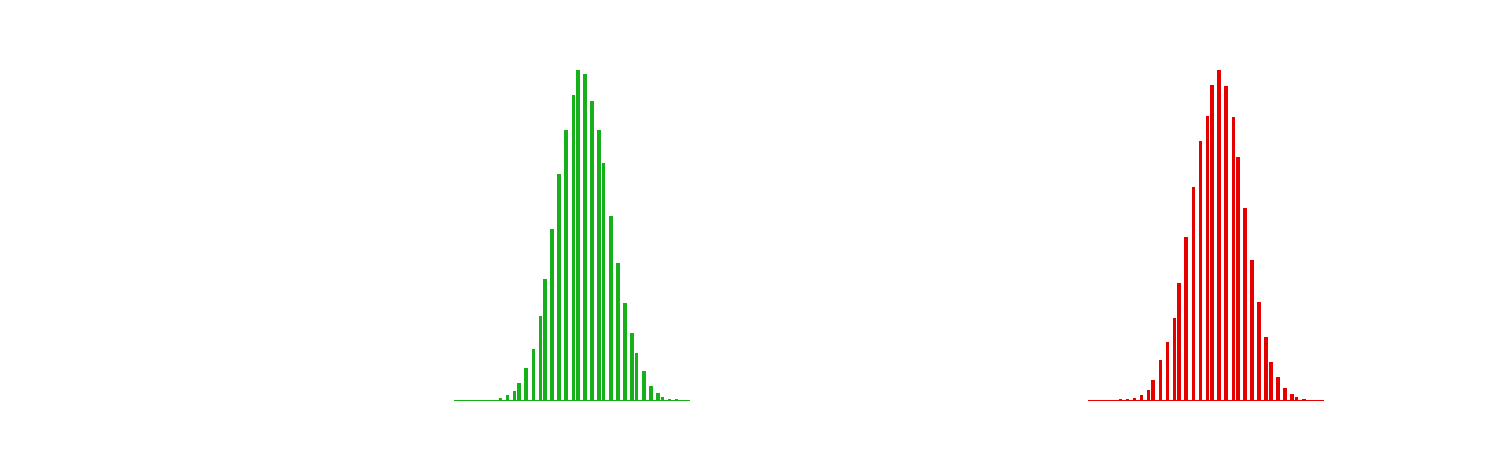
\includegraphics[width=\textwidth]{Results/3.5_boundariesBistability/maxReach0_0_HistogramPlot.pdf}
                    % \label{}
                \end{minipage}
            \end{minipage}
            \begin{minipage}{0.77\textwidth}
                \begin{minipage}{0.1\textwidth}
                    \caption*{\small \textbf{(b)}}
                \end{minipage}
                \begin{minipage}{0.66\textwidth}
                    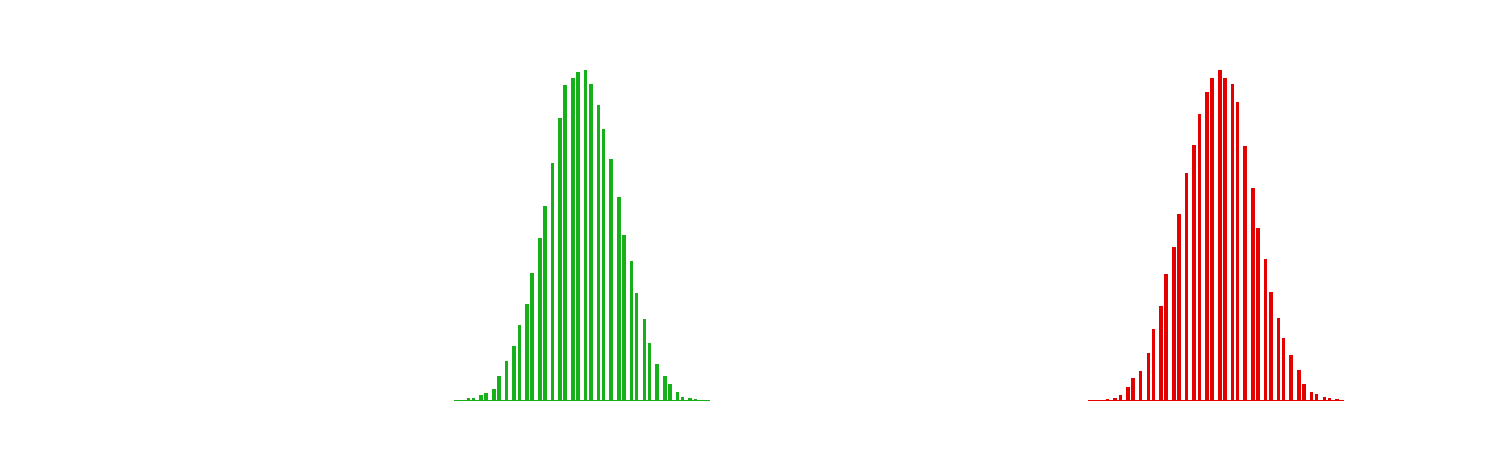
\includegraphics[width=\textwidth]{Results/3.5_boundariesBistability/maxReach1_4_HistogramPlot.pdf}
                \end{minipage}
            \end{minipage}
            \begin{minipage}{0.77\textwidth}
                \begin{minipage}{0.1\textwidth}
                    \caption*{\small \textbf{(c)}}
                    % \label{}
                \end{minipage}
                \begin{minipage}{0.66\textwidth}
                    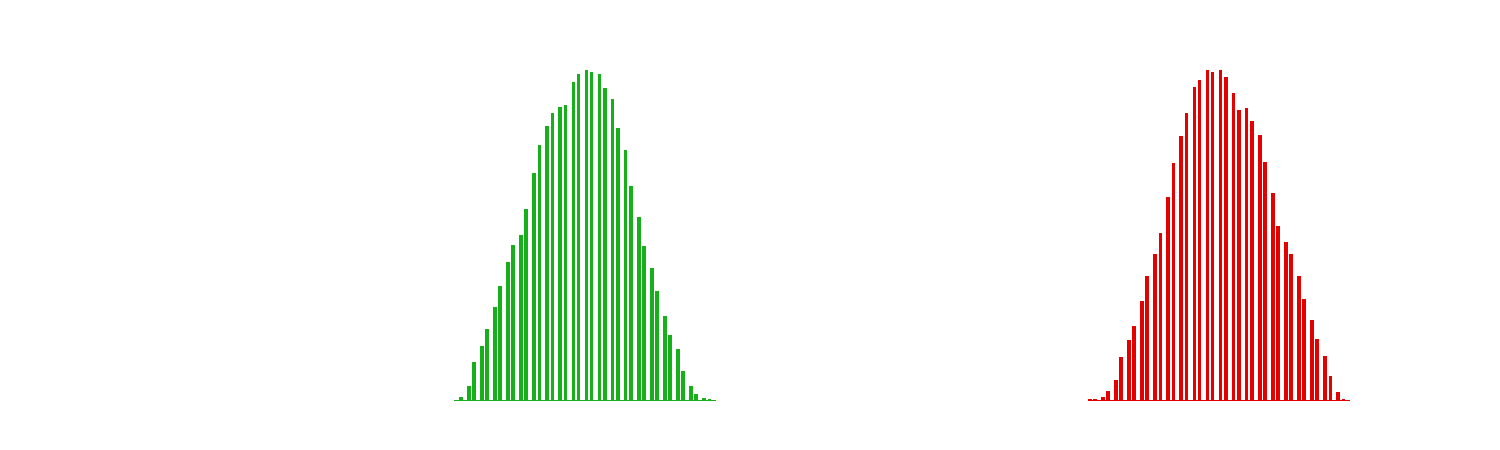
\includegraphics[width=\textwidth]{Results/3.5_boundariesBistability/maxReach2_2_HistogramPlot.pdf}
                    % \label{}
                \end{minipage}
            \end{minipage}
            \begin{minipage}{0.77\textwidth}
                \begin{minipage}{0.1\textwidth}
                    \caption*{\small \textbf{(d)}}
                \end{minipage}
                \begin{minipage}{0.66\textwidth}
                    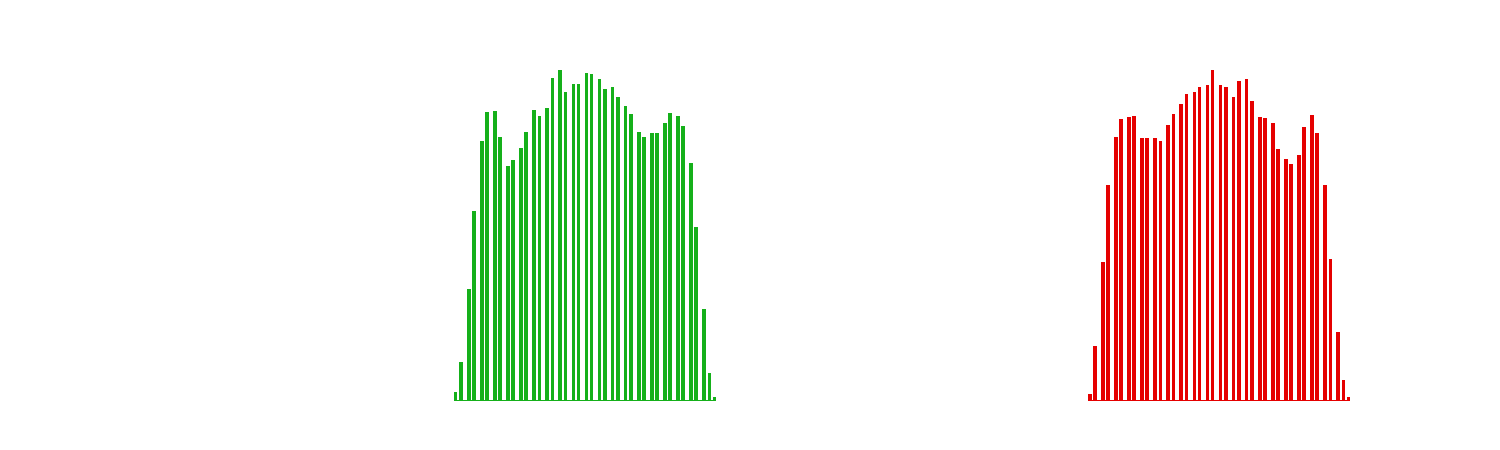
\includegraphics[width=\textwidth]{Results/3.5_boundariesBistability/maxReach3_3_HistogramPlot.pdf}
                \end{minipage}
            \end{minipage}
            \begin{minipage}{0.77\textwidth}
                \begin{minipage}{0.1\textwidth}
                    \caption*{\small \textbf{(e)}}
                    % \label{}
                \end{minipage}
                \begin{minipage}{0.66\textwidth}
                    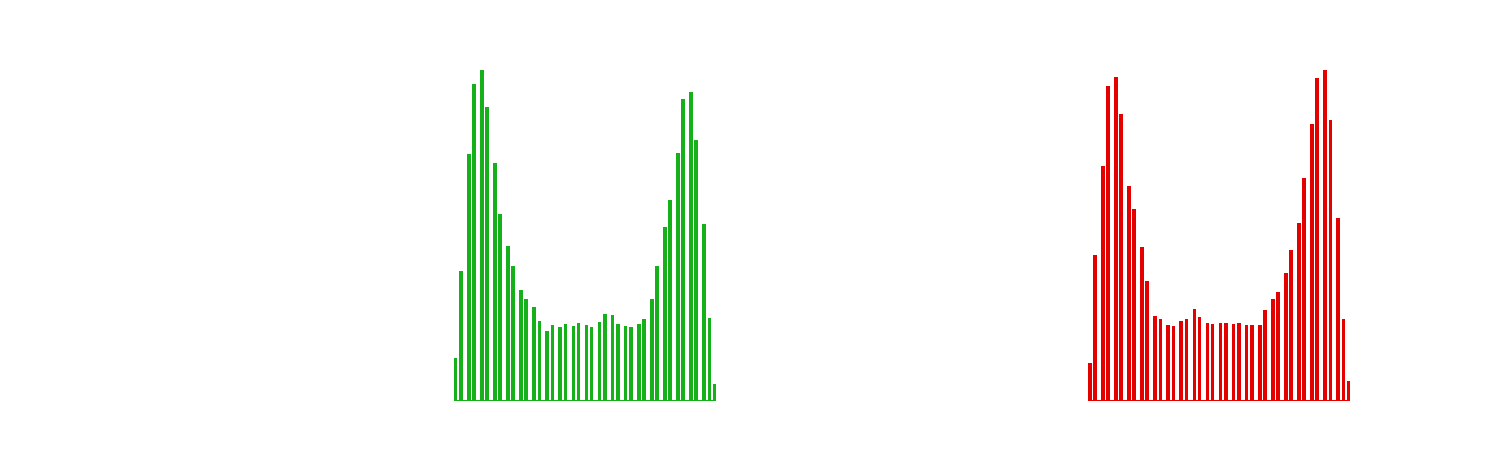
\includegraphics[width=\textwidth]{Results/3.5_boundariesBistability/maxReach4_3_HistogramPlot.pdf}
                    % \label{}
                \end{minipage}
            \end{minipage}
            \begin{minipage}{0.77\textwidth}
                \begin{minipage}{0.1\textwidth}
                    \caption*{\small \textbf{(f)}}
                \end{minipage}
                \begin{minipage}{0.66\textwidth}
                    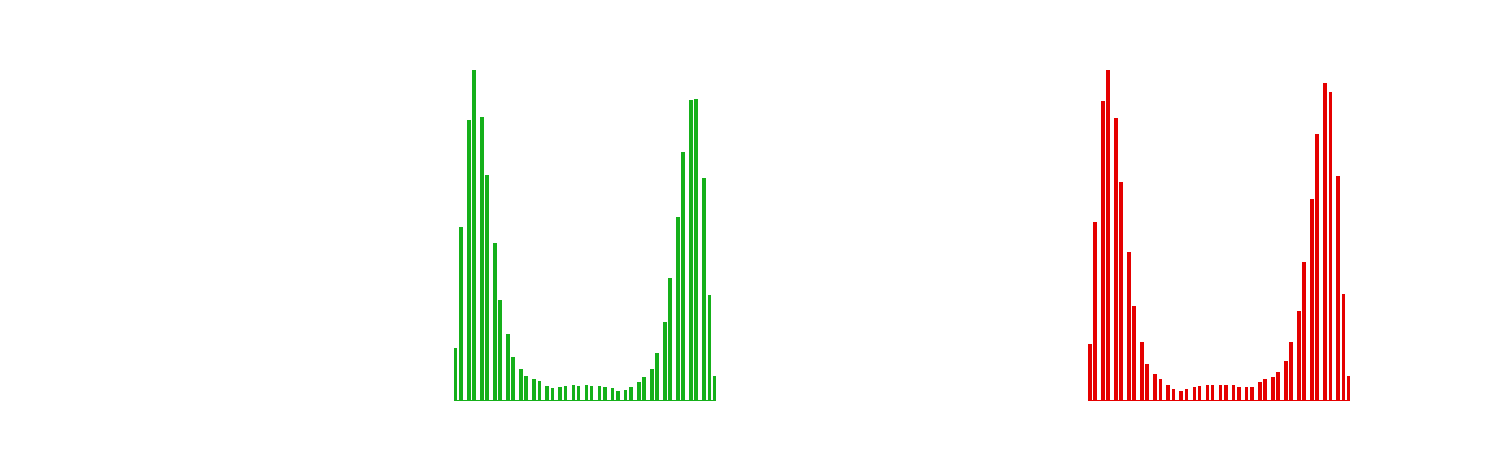
\includegraphics[width=\textwidth]{Results/3.5_boundariesBistability/maxReach5_4_HistogramPlot.pdf}
                \end{minipage}
            \end{minipage}
            \begin{minipage}{0.77\textwidth}
                \begin{minipage}{0.1\textwidth}
                    \caption*{\small \textbf{(g)}}
                \end{minipage}
                \begin{minipage}{0.66\textwidth}
                    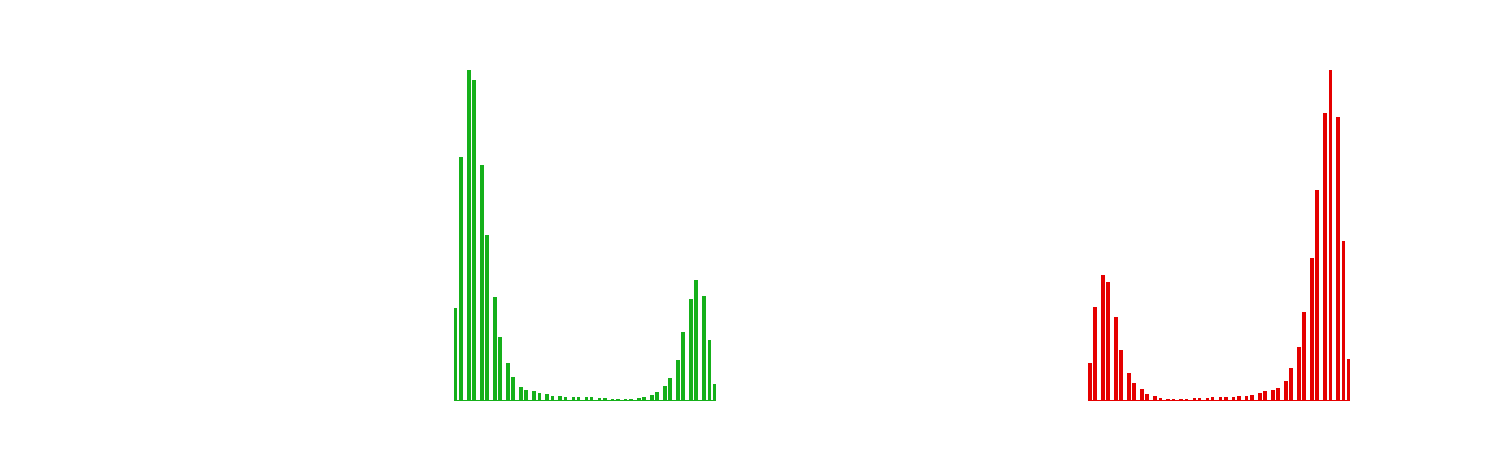
\includegraphics[width=\textwidth]{Results/3.5_boundariesBistability/maxReach6_4_HistogramPlot.pdf}
                \end{minipage}
            \end{minipage}
            \caption{}
            \label{img:enzymeReach}
        \end{figure}
        %
        \begin{itemize}
            {
                \color{red}
                \item describe loss of reach
                \item As can be seen in \textbf{(g)}, the symmetric case becomes more and more improbable because switching gets more rare and ?
            }
        \end{itemize}
        %
    %
    %
    \newpage
    \section{Bivalency} % TODO Should I include these  cases into the others above? Pro: I don't find anything ground-breaking here. Con: I have an entirely different system which might lead to confusion
        \label{sec:ResBivalency}
        %
        \begin{figure}[htpb!]
            \centering
            \includerunplot{Results/3.6_Bivalency/TotalComplete_example.png} % TODO change this
            \caption{}
            % \label{img:dissoc_runPlot2}
        \end{figure}
        %
        \begin{figure}[htpb!]
            \centering
            \includerunplot{Results/3.6_Bivalency/BivalentComplete_example.png} % TODO change this
            \caption{}
            % \label{img:dissoc_runPlot2}
        \end{figure}
        %
        \begin{figure}[htpb!]
            \centering
            \includerunplot{Results/3.6_Bivalency/BivalentBistability_example.png} % TODO change this
            \caption{}
            % \label{img:dissoc_runPlot2}
        \end{figure}
        %
        \begin{itemize}
            {
                \color{red}
                \item Here, we are at Kx+Ky
                \item Two systems that either favour bivalency or total active/silent states as an introduction to bivalency
                \item Frequent switching and bivalency
            }
        \end{itemize}
        %
    %
    %
%
%